\documentclass[tikz,border=2pt]{standalone}
\usepackage{tikz}
\usepackage{lmodern}
\usetikzlibrary{calc,decorations.pathreplacing}

% Visual conventions follow the existing MRNC TikZ pictures: ordinary
% components use TikZ's normal 0.4pt stroke, with compact TeX labels.
\tikzset{
  nu fibre/.style={
    x=0.78cm,
    y=0.78cm,
    line width=0.4pt,
    line cap=round,
    line join=round
  },
  nu label/.style={
    font=\scriptsize,
    inner sep=1pt
  },
  nu annotation/.style={
    font=\scriptsize,
    inner sep=1pt
  },
  nu dots/.style={
    font=\small,
    inner sep=0pt
  }
}



\begin{document}

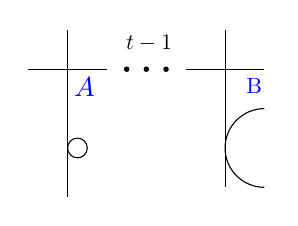
\begin{tikzpicture}[scale=0.5]
    \coordinate (C) at (-1.50, 3.00);
  \coordinate (D) at (-0.50, 3.00);
  \coordinate (A) at (-1.00, 3.00);
  \coordinate (B) at (-0.93, 3.26);

  \node[scale=0.8][above] at (B) {$t-1$};
  \fill[black] (C) circle (2pt);
  \fill[black] (D) circle (2pt);
  \fill[black] (A) circle (2pt);

  
  \coordinate (IIIrC) at (0.00, 3.00);
  \coordinate (IIIrD) at (2.00, 3.00);
  \coordinate (IIIrE) at (1.00, 4.00);
  \coordinate (IIIrF) at (1.00, 0.00);
  \coordinate (IIIrG) at (2.00, 1.00);
  \coordinate (IIIrD_1) at (1.74, 2.18);
  \draw (IIIrC) -- (IIIrD);
  \draw (IIIrE) -- (IIIrF);
  \draw (2.00, 2.00) arc (90.0:270.0:1.00);
  \node[scale=0.8][above, text=blue] at (IIIrD_1) {B};


\coordinate (A1) at (-4.00, 3.00);
  \coordinate (B1) at (-2.00, 3.00);
  \coordinate (C1) at (-3.00, 4.00);
  \coordinate (D1) at (-3.00, -0.25);
  \coordinate (E1) at (-2.75, 1.00);
  \coordinate (F1) at (-2.75, 1.00);
  \coordinate (G1) at (-2.57, 2.06);

  \draw (A1) -- (B1);
  \draw (C1) -- (D1);
  \draw (E1) circle (0.25);
  \node[above, text=blue] at (G1) {$A$};
  
\end{tikzpicture}

\end{document}
